\documentclass[english, 11pt]{article}
% \usepackage[T1]{fontenc}
% \usepackage[latin9]{inputenc}
\usepackage[top = 2cm, left = 2.5cm, right = 2.5cm, bottom = 2cm]{geometry}
\usepackage{enumitem}
% \usepackage{fontspec}
\usepackage{amsmath}
\usepackage{amsfonts}
\usepackage{amstext}
\usepackage{mdframed}
\usepackage{graphicx}
\usepackage{wrapfig}
% \usepackage{bbm}
\makeatletter
\@ifundefined{date}{}{\date{}}
\usepackage{tikz}
\usetikzlibrary{quotes, angles, decorations.markings, intersections}
\usetikzlibrary{calc,patterns,angles,quotes, 3d, intersections, positioning, shapes, automata, positioning}
\usepackage{wasysym}
\makeatother
\usepackage{babel}
\usepackage{color}
\usepackage{graphicx}
\usepackage{hyperref}
\hypersetup{
	colorlinks,
	citecolor=black,
	filecolor=black,
	linkcolor=black,
	urlcolor=black
}


\newcommand{\tbox}[1]{\noindent\fbox{\parbox{\textwidth}{#1}}}

\setlength{\parindent}{0pt}

\begin{document}

\textbf{CS 745 : Principles of Data and System Security} \hfill
\textit{Scribed by}: Kavin Arvind and Nikil S

\noindent\tbox{

\begin{center}
  \huge Lecture - 01 \\ % change lecture number
  \Large Topic:  History of Cryptography
\end{center}

}

\section*{Shifted cipher}
Each letter is Shifted by $k$ and sent. Eg- "A" is written as "A"+k (Shifted by k letters) and sent. \\
This is easy to decode as only 26 ( or 36 (if 0-9 nos are included)) possible $k$ are there and thus its easy to check each possibility.

\section*{Rolling by wooden stick}
A paper is rolled on to a stick and text is written. If seen normally, the letters would look fully shuffled, but if its rolled in the same way as it was written, it can be decoded.\\
eg- "MY NAME IS X" is written like
\begin{figure}[ht]
    \centering
        \begin{tabular}{ccccccccc}
            M &   &   &   & M &   &   &   & X\\
              & Y &   & A &   & E &   & S &  \\
              &   & N &   &   &   & I &   &  \\
        \end{tabular}
\end{figure}
\\
Thus its crypted as MMXYAESNI.

\section*{Mono-Substitution cipher}
We have a table where each letter is mapped to other letters and text is ciphered according to that. Here, we have here $26!$ ways of mapping and so its very difficult to try different possibilities. \\
This seems like an optimal solution, but there is a problem. In an average english text, each letter has a specific frequency of repetition. \\
Say letter "A" is coded to letter "K" (randomly). So frequency of letter K would be same as of the letter "A" in a normal text. So by this way, cipher text could possibly be decrypted.

\clearpage
\noindent\tbox{

\begin{center}
  \huge Lecture - 02 \\ % change lecture number
  \Large Topic:  History of Cryptography(Continuation.)
\end{center}

}

\section*{Homophonic Cipher}
The main problem of Mono-Substitution cipher is that, a character was substituted with only one alphabet and so the frequency didn't change.\\
What if its substituted with many characters to equalize the frequencies? \\
Say $S = \{A,B,..Z,0,1,..9,\epsilon, \alpha, \beta, \gamma, ...\}$ has usable symbols. \\
Say letter "A" has frequency $x\%$. We allot $\frac{x}{100} \times |S|$ number of symbols and are randomly substituted in the cipher text in place of "A".
This uniforms/balences the frequency among all the symbols and hence difficult to decrypt by frequency method. \\
But here, storing the mapping, encrypting, and decrypting are difficult.

\section*{Vigenere's Cipher}

What if we substitute "A" by any of the letters strategically? Vigenere created a table as shown below.

\begin{figure}[ht]
  \centering
      \begin{tabular}{|c|c|c|c|c|c|c|c|c|}
          \hline
            & A & B & C & D & ..\\
          \hline
          A & B & C & D & E & ..\\
          B & C & D & E & F & ..\\
          . &   &   &   &   &   \\
          . &   &   &   &   &   \\
          \hline
      \end{tabular}
\end{figure}
A keyword is chosen and correspondingly added to the text encrypt it. Eg -
\begin{figure}[ht]
  \centering
      \begin{tabular}{|c|ccccccccc|}
          \hline
          Actual text & M & Y & N & A & M & E & I & S & X \\
          keyword     & R & O & S & E & R & O & S & E & R \\
          \hline
          Cipher      & .. &   &   & F &   &   &   &   & \\
          \hline
      \end{tabular}
\end{figure}
Thus here, according to the position, same letter is encrypted to different letters and thus the frequencies are balenced.\\
Is it a good method then? \\
Words like "THE", "IS", etc repeat so much in english that its very likely that it is encrypted to the same cipher text due to same relative position w.r.t keyword. Calculating the repeated strings in ciphertext and observing the distance between them will give insigts about the length of keyword.
Length of keyword would be a factor of those distances and can be found out(say $l$). Now, characters $1,1+l,1+2l,..$ are derived from same column of the table. Hence they are like monostituted and now, frequencies can be calculated out to find the keyletters and hence keyword.

\section*{Mordern Cryptography}
\subsection*{Shannon's Cipher}
$\xi = (E,D)$ is a cipher system where $E(m,k) = c$($m$ is message, $k$ is key, $c$ is cipher text) is encyption funtion, and $D(c,k) = m$ is decryption funtion.

\subsection*{One Time Pad}
Say $m^l$ is a message of bits of length $l$, and key $k^l$ is key of same length generated randomly.
\[ E(m,k)= m^l \oplus k^l = c \]
\begin{align*}
  D(c,k) &= c^l \oplus k^l \\
  &= m^l \oplus k^l \oplus k^l \\
  &= m^l \\
\end{align*}
Provided key is generated completely random, and no part of key is known to Evasdropper, they can't decrypt it as probability of $c$ being 0 or 1 is independent of message itself. I.e,
\[ Prob(cipher = c | msg = m) = Prob(cipher = c | msg = m') \]
Hence, it is safe.
Disadvantages:
\begin{itemize}
  \item key is as big as message(or more)
  \item key should be sent safely. Otherwise its easily decrypted.
\end{itemize}
If key length is more, either its padded at the end and xored, or key is taken till the length of message and xored. \\
In general, if its not a bit string, the encryption can be taken as sum modulus like:
\[ E(m,k)= m^l + k^l \pmod{n} = c \text{  (if n=2, its just xor)} \]
\begin{align*}
  D(c,k) &= c^l - k^l \pmod{n} \\
  &= m^l + k^l - k^l \pmod{n}\\
  &= m^l \pmod{n}\\
\end{align*}

\clearpage
\noindent\tbox{

\begin{center}
  \huge Lecture - 03 \\ % change lecture number
  \Large Topic:  Perfect Secrecy and Shannon's information Theory
\end{center}

}
\section*{Perfectly secrecy}
\subsection*{OTP}
For a message to be perfectly secret, the Evasdropper should not be able to get any extra information from the ciphertext. So, \\
\begin{align*}
  P(M=m|C=c) &= P(M=m) \quad \text{[message = m, and ciphertext = c]} \\
  P_c(m) &= P(m) \\
  \frac{P(M=m|C=c)}{P(M=m)} &= \frac{P(C=c|M=m)}{P(C=c)} \\
  &= \frac{P(C=c|M=m)}{\sum_{m' \in M} P(C=c|M=m')P(M=m')} \\
\end{align*}
\[
\left[
\begin{aligned}
  P(C=c|M=m') &= P(K \oplus m' = c | M = m') \\
  &= P(K = c \oplus m'  | M = m') \\
  &= \frac{1}{2^l} \quad \text{[as key is selected randomly, probability that its $c \oplus m'$ is $1/2^l$]} \\
\end{aligned}
\right]
\]
\begin{align*}
  \frac{P(M=m|C=c)}{P(M=m)} &= \frac{P(C=c|M=m)}{\sum_{m' \in M} P(C=c|M=m')P(M=m')} \\
  &= \frac{1/2^l}{\sum_{m' \in M} (1/2^l)P(M=m')} \\
  &= \frac{1}{\sum_{m' \in M} P(M=m')} \\
  &= \frac{1}{1} \\
  P(M=m|C=c) &= P(M=m) \\
\end{align*}
Hence proved that it is perfectly secret. \\
But, what happens if key is repeated? Say a message said "Fire the gun" to a soldier which was ciphered to $c$ using key $k$, though an Evasdropper technically doesn't know the key, now he would see the soldier firing after getting message and so he can guess the message.
Using the ciphertext, he can get the $key = message \oplus cipher$ and if same key is used again, he would guess the message. Thus key can be used just once.\\
Also, if $M = {m_1='a',m_2='ab'}$ and,\\
if $c='x'$, $P_c(m_1) = 1$ and $P_c(m_2) = 0$ (This method reveals length of the message) \\
if $c='xy'$, $P_c(m_1) = 0$ and $P_c(m_2) = 1$.

\subsection*{Substitution cipher}
If $M = {m_1='aa',m_2='ab'}$ and,\\
if $c='xx'$, $P_c(m_1) = 1$ and $P_c(m_2) = 0$. \\
if $c='xy'$, $P_c(m_1) = 0$ and $P_c(m_2) = 1$. \\
Thus its not perfectly secret.

\subsection*{Addition OTP}

\begin{align*}
  D(c,k) &= c^l - k^l \pmod{n} \\
  &= m^l + k^l - k^l \pmod{n}\\
  &= m^l \pmod{n}\\
\end{align*}
Proof is very similar to as OTP.

\section*{Shannon's information Theory}
"No class on Friday" has more information/importance than "There is class on Friday" because having no class is a rare thing, and need to informed importantly. Having class is a regular thing and it doesn't carry much info.
So,
\begin{align*}
  \text{information} &\propto \frac{1}{\text{probability of occurance}} \\
  Info(x) &\propto \frac{1}{P(x)} \\
\end{align*}
Entropy of a message distibution($X$) is defined as:
\begin{align*}
  H(X) &= -\sum_{x \in X} P(x) \log_{2}(P(x)) \\
  &= \sum_{x \in X} P(x) \log_{2}(\frac{1}{P(x)}) \\
\end{align*}
Entropy is max when each of the messages has equal probability i.e, they are more uncertain. \\
Conditonal entropy of X, given Y is:
\begin{align*}
  H_Y(X)&= \sum_{X,Y} P(x,y) \log_{2}(\frac{1}{P_y(x)}) \\
  &= \sum_{Y} P(y) \sum_{X} P(x) \log_{2}(\frac{1}{P_y(x)}) \\
\end{align*}
If $C$ is the cipher text, and if $ H_C(M) \approx 0 $, then its easily breakable as it is not that uncertain.

\clearpage
\noindent\tbox{

\begin{center}
  \huge Lecture - 04 \\ % change lecture number
  \Large Topic: Key distributions
\end{center}

}

\section*{Symmetric Key Cryptography}
The methods we have seen so far including Substitution cipher, OTP, etc, are Symmetric key Cryptography as both the sender and receiver needs the same key to encrypt and decrypt the message. Here, the main difficulty was to exchage keys between both parties safely.\\
Its two types are \textbf{Stream Cipher} and \textbf{Block cipher} which we'll see later.

\section*{Assymetric key Cryptography}

Here, a pair of Keys $E_k$ and $D_k$ are created by a party which are related to each other in some sense.\\

\subsection*{Method 1: Secrecy Ensured}
Lets say, person $A$ wants to send a message to person $B$. Now, person $B$ created the pair of keys $E_B$ and $D_B$ and sends $E_B$ publically.
So, now $A$ encrypts message $m$ using $E_B$ to send cipher $c$.\\
Here, since $D_B$ is known only by person $B$, just $B$ can decrypt it and no one else. Thus here, secracy is ensured. But, cipher $c$ can be tapped and some other message $m'$ can be encrypted to $c'$ using public key $E_B$ by an Evasdropper and sent. So, here, authenticity is not ensured.

\begin{figure}[ht]
  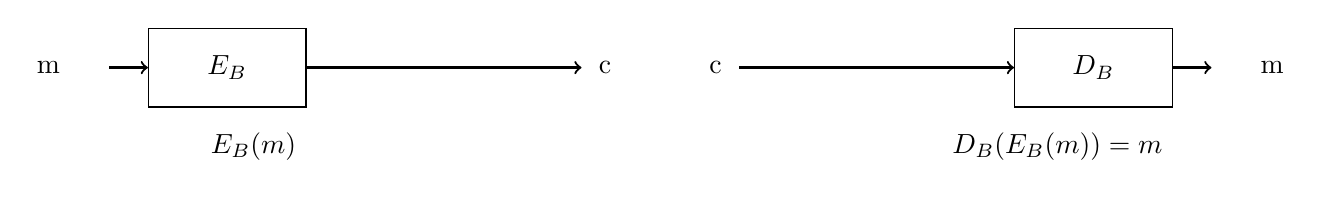
\begin{tikzpicture}
    % First set of text and boxes
    \node[anchor=east] at (0,0) {m};
    \node[draw, rectangle, minimum width=2cm, minimum height=1cm] (box1) at (2,0) {$E_B$};
    \node[anchor=east] at (3,-1) {$E_B(m)$};
    \node[anchor=west] at (8,0) {c};

    % Arrows
    \draw[->, thick] (0.5,0) -- (box1.west);
    \draw[->, thick] (box1.east) -- (6.5,0);

    % Second set of text and boxes
    \node[anchor=east] at (7,0) {c};
    \node[draw, rectangle, minimum width=2cm, minimum height=1cm] (box4) at (13,0) {$D_B$};
    \node[anchor=east] at (14,-1) {$D_B(E_B(m)) = m$};
    \node[anchor=west] at (15,0) {m};

    % Arrows
    \draw[->, thick] (8.5,0) -- (box4.west);
    \draw[->, thick] (box4.east) -- (14.5,0);

\end{tikzpicture}


  \centering   
\end{figure}

\subsection*{Method 2: Authenticity Ensured}
Lets say, person $A$ wants to send a message to person $B$. Now, person $A$ created the pair of keys $E_A$ and $D_A$ and sends $E_A$ publically.
So, now $A$ encrypts message $m$ using $D_A$ to send cipher $c$.\\S
Here, since $E_A$ is known by everyone including $B$, he can decrypt it using $E_A$. Thus here, authenticity is ensured as $D_A$ is private to person $A$ and only he/she can encrypt it. But, cipher $c$ can be decrypted by littrally everyone as $E_A$ is known publically. So security is not ensured.

\begin{figure}[ht]
  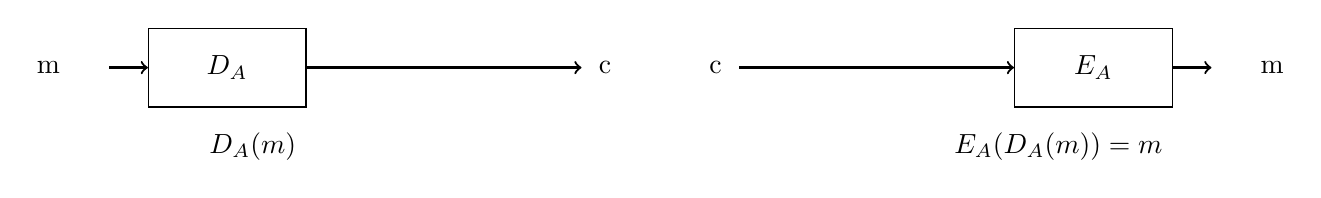
\begin{tikzpicture}
    % First set of text and boxes
    \node[anchor=east] at (0,0) {m};
    \node[draw, rectangle, minimum width=2cm, minimum height=1cm] (box1) at (2,0) {$D_A$};
    \node[anchor=east] at (3,-1) {$D_A(m)$};
    \node[anchor=west] at (8,0) {c};

    % Arrows
    \draw[->, thick] (0.5,0) -- (box1.west);
    \draw[->, thick] (box1.east) -- (6.5,0);

    % Second set of text and boxes
    \node[anchor=east] at (7,0) {c};
    \node[draw, rectangle, minimum width=2cm, minimum height=1cm] (box4) at (13,0) {$E_A$};
    \node[anchor=east] at (14,-1) {$E_A(D_A(m)) = m$};
    \node[anchor=west] at (15,0) {m};

    % Arrows
    \draw[->, thick] (8.5,0) -- (box4.west);
    \draw[->, thick] (box4.east) -- (14.5,0);

\end{tikzpicture}


  \centering   
\end{figure}

\subsection*{Method 3: Both Ensured}
What if we combine both the above methods to ensure both..\\
Lets say, person $A$ wants to send a message to person $B$.\\
Both of them creates pairs of keys $E_A$, $D_A$ and $E_B$, $D_B$ (and, $E_B$, $E_A$ are public).

\begin{figure}[ht]
  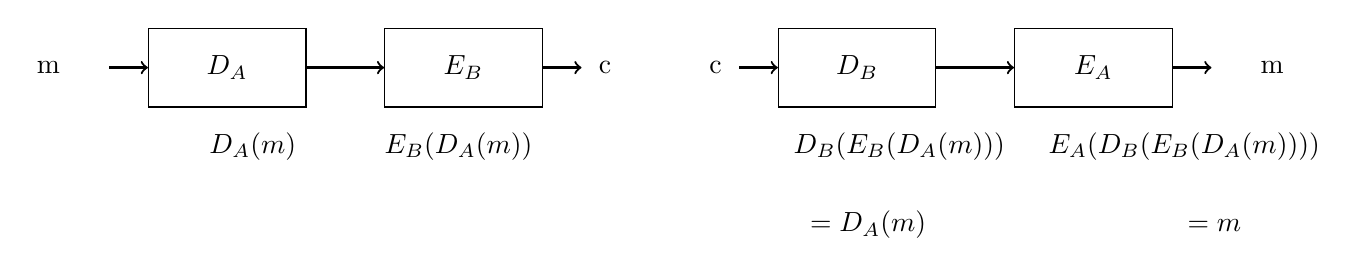
\begin{tikzpicture}
    % First set of text and boxes
    \node[anchor=east] at (0,0) {m};
    \node[draw, rectangle, minimum width=2cm, minimum height=1cm] (box1) at (2,0) {$D_A$};
    \node[anchor=east] at (3,-1) {$D_A(m)$};
    \node[draw, rectangle, minimum width=2cm, minimum height=1cm] (box2) at (5,0) {$E_B$};
    \node[anchor=east] at (6,-1) {$E_B(D_A(m))$};
    \node[anchor=west] at (8,0) {c};

    % Arrows
    \draw[->, thick] (0.5,0) -- (box1.west);
    \draw[->, thick] (box2.east) -- (6.5,0);

    % Second set of text and boxes
    \node[anchor=east] at (7,0) {c};
    \node[draw, rectangle, minimum width=2cm, minimum height=1cm] (box3) at (10,0) {$D_B$};
    \node[anchor=east] at (12,-1) {$D_B(E_B(D_A(m)))$};
    \node[anchor=east] at (11,-2) {$ = D_A(m)$};
    \node[draw, rectangle, minimum width=2cm, minimum height=1cm] (box4) at (13,0) {$E_A$};
    \node[anchor=east] at (16,-1) {$E_A(D_B(E_B(D_A(m))))$};
    \node[anchor=east] at (15,-2) {$ = m$};
    \node[anchor=west] at (15,0) {m};

    % Arrows
    \draw[->, thick] (8.5,0) -- (box3.west);
    \draw[->, thick] (box4.east) -- (14.5,0);
    \draw[->, thick] (box1.east) -- (box2.west);
    \draw[->, thick] (box3.east) -- (box4.west);

\end{tikzpicture}


  \centering   
\end{figure}
This suffices both authenticity and secracy. Here, its noteworthy that algorithm is known by everyone unlike the historical methods and just that the keys are kept secret.

\section*{Access Control}
Eg- MAC, DAC, RBAC, ABAC, etc are algorithms/methods used to enable access control. Lets understand this with an eg: \\
Lets say there is data stored in a database where only specific users can read and special users can edit it. Also, people should not be able to delete or scatter the information.
So, readers and modifiers should have their own specific keys.

\section*{Random Number Generation}
Its of two types:
\subsection*{True Random Number generator(TRNG)}
This is based on actual random events such as some hardware that changes drastically with outside conditions. It is truely random and can't be predicted.

\subsection*{Pseudo Random Number generator(PRNG)}
This is done algorithmic and could be predicted based on its previous values.

% 25 - 01 - 2024 LECTURE 5
\clearpage
\noindent\tbox{
\begin{center}  
    \huge Lecture - 05 \\
    \Large Topic: Symmetric Crytopgraphy(Stream Cipher, LFSR)
\end{center}
}

\section*{Weekly Test 1 Solutions}
\subsection*{Question 2}
Given : \\
Length of code = 128 bits \\
Cost of a processor = Rs.1000 \\
Cap on cost of processors is Rs.10 crores. The performance of the processors is 10ns/code and follows Moore's law, i.e. it doubles in 24 months. The code is expected to be broken in 7 days. \\ \\
Solution: \\
In $n$ years, performance will increase by a factor of $2^{\frac{n}{2}}$. Therefore, 
\[
2^{128} codes \times \frac{10\times 10^{-9}s}{2^{\frac{n}{2}}} = \frac{10 crore}{1000} processors \times 7days \times 24hrs \times 60min \times 60s
\]
On solving, $n$ turns out to be approximately 130 years.

\section*{Symmetric Encryption: Stream Cipher}
The input is a stream of bits and the encryption takes place one bit at a time. It is easy to compute. \\ 
e.g.: One Time Pad which encrypts as follows
\begin{gather*}
    c_{i} = m_{i} \oplus k_{i} \\
    c_{i} = m_{i} + k_{i} \bmod 2
\end{gather*}

To use this encryption we need a random number generator to obtain k. True random numbers can be generated from physical phenomena. Rather, We are gonna generate pseudo-random numbers, i.e., random numbers generated algorithmically. One such method is LFSR.

\subsection*{Linear Feedback Shift Register}

LFSR is a shift register whose input bit is a \textbf{linear} function of two or more of the previous output bits.

\begin{figure}[ht]
\begin{center}
      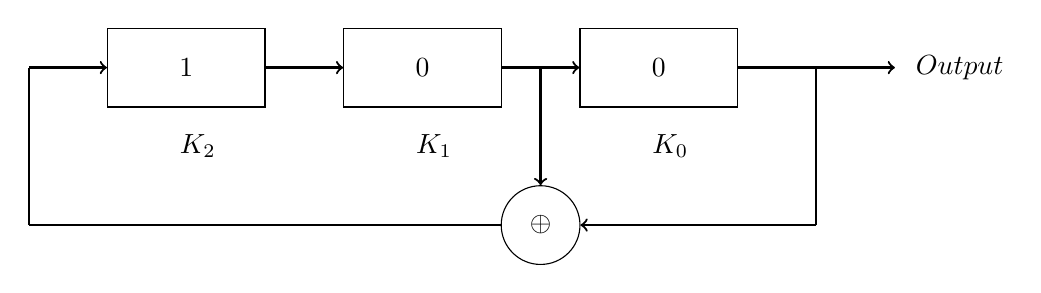
\begin{tikzpicture}
    % First set of text and boxes
    \node[draw, rectangle, minimum width=2cm, minimum height=1cm] (box1) at (2,0) {1};
    \node[anchor=east] at (2.5,-1) {$K_{2}$};
    \node[draw, rectangle, minimum width=2cm, minimum height=1cm] (box2) at (5,0) {0};
    \node[anchor=east] at (5.5,-1) {$K_{1}$};
    \node[draw, rectangle, minimum width=2cm, minimum height=1cm] (box3) at (8,0) {0};
    \node[draw, circle, minimum size=1cm] (xor1) at (6.5,-2) {$\oplus$};
    \node[anchor=east] at (8.5,-1) {$K_{0}$};
    \node[anchor=east] at (12.5,0) {$Output$};


    % Arrows
    \draw[->, thick] (0,0) -- (box1.west);
    \draw[->, thick] (box1.east) -- (box2.west);
    \draw[->, thick] (box2.east) -- (box3.west);
    \draw[->, thick] (box3.east) -- (11,0);
    \draw[-, thick] (10,0) -- (10,-2);
    \draw[->, thick] (10,-2) -- (xor1.east);
    \draw[->, thick] (6.5,0) -- (xor1.north);
    \draw[-, thick] (xor1.west) -- (0,-2);
    \draw[-, thick] (0,-2) -- (0,0);

\end{tikzpicture}
\end{center}

  \centering   
\end{figure}

The sequence generated by the given circuit is 
\begin{gather*}
    K_{i+3} = K_{i+1} \oplus K_{i} \\
    K_{i+3} = K_{i+1} + K_{i} \bmod 2\\
\end{gather*}
The expression for the input bit of an LFSR can be represented by a polynomial of degree $n$ ($n$ = number of registers), known as the characteristic polynomial. For example, the polynomial of the above LFSR circuit is
\begin{gather*}
x^{3} = x + 1 \bmod 2 \\
x^{3} + x + 1 \bmod 2 =0
\end{gather*}
Such a polynomial is called primitive if it is a factor of $x^{2^{n}-1}+1 \bmod 2$. A primitve polynomial generates a maximum length cycle of register values for given number of registers (cycle length = $2^{n}-1$, every pattern except 0). For example, the above polynomial generates the following series:\\
\[
100, 010, 101, 110, 111, 011, 001 
\]
of length $2^{3}-1 = 7$. Note that the polynomial is a factor of $x^{7}+1 \bmod 2$.
\[x^{2^{n}-1}+1 \bmod 2 = (x + 1)\times (x^{3} + x + 1)\times (x^{3} + x^{2} + 1)\bmod 2\]
To preserve randomness, the length of the cycle should be maximized, and so a primitive polynomial is preferred. Otherwise, we will end up generating a cyle of length less than $2^{n}-1$.\\

Here, the key depends on 
\begin{itemize}
    \item Characteristic polynomial
    \item \textbf{Seed} (Initial Value of the registers)
\end{itemize}

\subsection*{Programmable LFSR}
An LFSR circuit of degree $n$ that can configured to adopt any characteristic polynomial of the same degree. Here's an example of a programmable LFSR of degree 4.

\begin{center}
      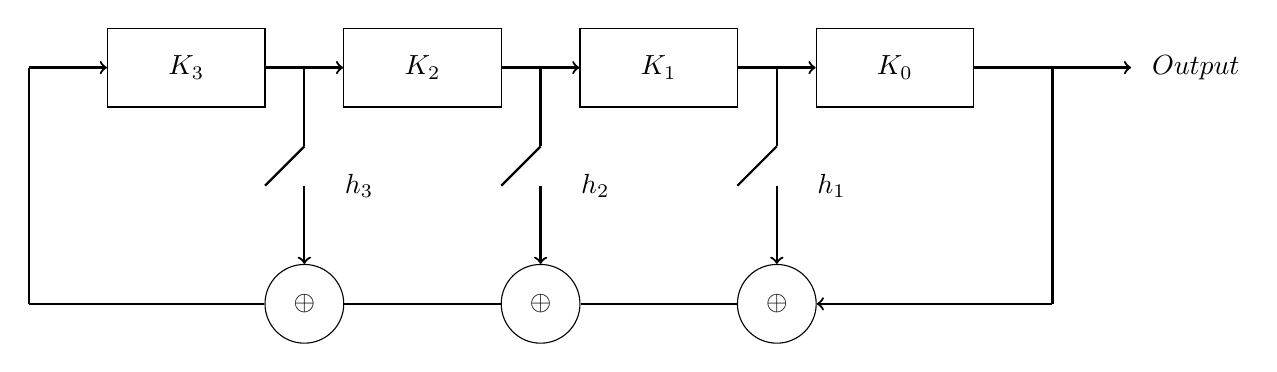
\begin{tikzpicture}
    % First set of text and boxes
    \node[draw, rectangle, minimum width=2cm, minimum height=1cm] (box1) at (2,0) {$K_{3}$};
    \node[anchor=east] at (4.5,-1.5) {$h_{3}$};
    \node[draw, rectangle, minimum width=2cm, minimum height=1cm] (box2) at (5,0) {$K_{2}$};
    \node[anchor=east] at (7.5,-1.5) {$h_{2}$};
    \node[draw, rectangle, minimum width=2cm, minimum height=1cm] (box3) at (8,0) {$K_{1}$};
    \node[anchor=east] at (10.5,-1.5) {$h_{1}$};
    \node[draw, rectangle, minimum width=2cm, minimum height=1cm] (box4) at (11,0) {$K_{0}$};
    \node[draw, circle, minimum size=1cm] (xor1) at (9.5,-3) {$\oplus$};
    \node[draw, circle, minimum size=1cm] (xor2) at (6.5,-3) {$\oplus$};
    \node[draw, circle, minimum size=1cm] (xor3) at (3.5,-3) {$\oplus$};
    \node[anchor=east] at (15.5,0) {$Output$};


    % Arrows
    \draw[->, thick] (0,0) -- (box1.west);
    \draw[->, thick] (box1.east) -- (box2.west);
    \draw[->, thick] (box2.east) -- (box3.west);
    \draw[->, thick] (box3.east) -- (box4.west);
    \draw[->, thick] (box4.east) -- (14,0);
    \draw[-, thick] (13,0) -- (13,-3);
    \draw[->, thick] (13,-3) -- (xor1.east);
    % tap1
    \draw[-, thick] (9.5,0) -- (9.5,-1);
    \draw[-, thick] (9.5,-1) -- (9,-1.5);
    \draw[->, thick] (9.5,-1.5) -- (xor1.north);
    % tap2
    \draw[-, thick] (6.5,0) -- (6.5,-1);
    \draw[-, thick] (6.5,-1) -- (6,-1.5);
    \draw[->, thick] (6.5,-1.5) -- (xor2.north);
    % tap3
    \draw[-, thick] (3.5,0) -- (3.5,-1);
    \draw[-, thick] (3.5,-1) -- (3,-1.5);
    \draw[->, thick] (3.5,-1.5) -- (xor3.north);
    \draw[-, thick] (xor1.west) -- (xor2.east);
    \draw[-, thick] (xor2.west) -- (xor3.east);
    \draw[-, thick] (xor3.west) -- (0,-3);
    \draw[-, thick] (0,-3) -- (0,0);

\end{tikzpicture}
\end{center}
The sequence generated by this would depend on the keys h1,h2,h3 as shown:
\begin{gather*}
        K_{i+4} = h_{3}K_{i+3} + h_{2}K_{i+2} + h_{1}K_{i+1} + K_{i} \bmod 2\\
\end{gather*}
Due to its linear nature, an LFSR can be easily broken.
We shall introduce non-linearity by using AND and OR gates in the circuit which will be covered in the next class :)

% 29 - 01 - 2024 LECTURE 6
\clearpage
\noindent\tbox{
\begin{center}  
    \huge Lecture - 06 \\
    \Large Topic: DES, Feistel Cipher
\end{center}
}

\section*{Stream Cipher - Short Summary}

\begin{figure}[ht]
\begin{center}
\begin{tikzpicture}
      % First set of text and boxes
      \node[draw, circle, minimum size=1cm] (xor1) at (2,-2) {$\oplus$};
      \node[anchor=east] at (0,-2) {$m$};
      \node[anchor=north] at (2,0) {$k_{i}$};
      \node[anchor=west] at (4,-2) {$c_{i}$};
  
  
      % Arrows
      \draw[->, thick] (0,-2) -- (xor1.west);
      \draw[->, thick] (xor1.east) -- (4,-2);
      \draw[->, thick] (2,-0.5) -- (xor1.north);
  
\end{tikzpicture}
\end{center}

  \centering   
\end{figure}

\section*{Block Cipher}
Bundle of bits are fed. %\hfill DES

\begin{figure}[ht]
  \begin{center}
  \begin{tikzpicture}
        % First set of text and boxes
        \node[draw, rectangle, minimum width=2cm, minimum height=1cm] (box) at (2,-2) {};
        \node[anchor=east] at (0,-2) {$m$};
        \node[anchor=north] at (2,0) {$k$};
        \node[anchor=west] at (4,-2) {$c$};

        % DES
        \node[draw, rectangle, minimum width=2cm, minimum height=1cm] (box2) at (10,-2) {DES};
        \node[anchor=south] at (8,-2) {$m$};
        \node[anchor=north] at (8,-2) {64 $bit$};
        \node[anchor=south] at (10,0) {$k$};
        \node[anchor=north] at (10,0) {56 $bit$};
        \node[anchor=south] at (12,-2) {$c$};
        \node[anchor=north] at (12,-2) {64 $bit$};

        % Arrows
        \draw[->, thick] (0,-2) -- (box.west);
        \draw[->, thick] (box.east) -- (4,-2);
        \draw[->, thick] (2,-0.5) -- (box.north);
        % Arrows des
        \draw[->, thick] (8.5,-2) -- (box2.west);
        \draw[->, thick] (box2.east) -- (11.5,-2);
        \draw[->, thick] (10,-0.5) -- (box2.north);
    
  \end{tikzpicture}
  \end{center}
  
    \centering   
  \end{figure}

\subsection*{Principle}
\begin{figure}[ht]
  \begin{center}
  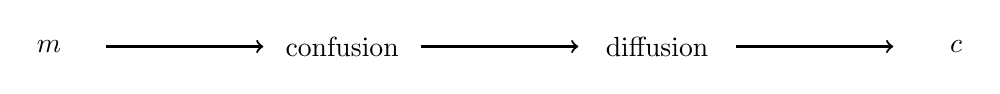
\begin{tikzpicture}
        % First set of text and boxes
        \node[anchor=west] at (0,0) {$m$};
        \node[anchor=center] at (4,0) {confusion};
        \node[anchor=center] at (8,0) {diffusion};
        \node[anchor=east] at (12,0) {$c$};
        % Arrows
        \draw[->, thick] (1,0) -- (3,0);
        \draw[->, thick] (5,0) -- (7,0);
        \draw[->, thick] (9,0) -- (11,0);
  \end{tikzpicture}
  \end{center}
  
    \centering   
  \end{figure}

% WRAPFIG
\begin{wrapfigure}{r}{0.5\textwidth}
  \begin{flushright}
    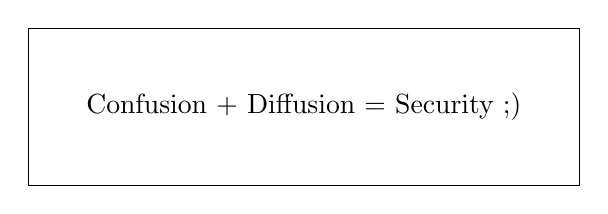
\begin{tikzpicture}
      \draw (0,0) rectangle (7,2);
      \node at (3.5,1) {Confusion + Diffusion = Security ;)};
    \end{tikzpicture}
    %\caption{Your TikZ figure caption here.}
  \end{flushright}
\end{wrapfigure}

The text undergoes several iterations of confusion and diffusion.

\subsubsection*{Confusion}
Relation between the text message and ciphertext is obscure.

\subsubsection*{Diffusion}
Change in one bit in the plaintext influences multiple bits in the ciphertext.

\vspace*{20pt}

\begin{figure}[h!]
  \begin{center}
  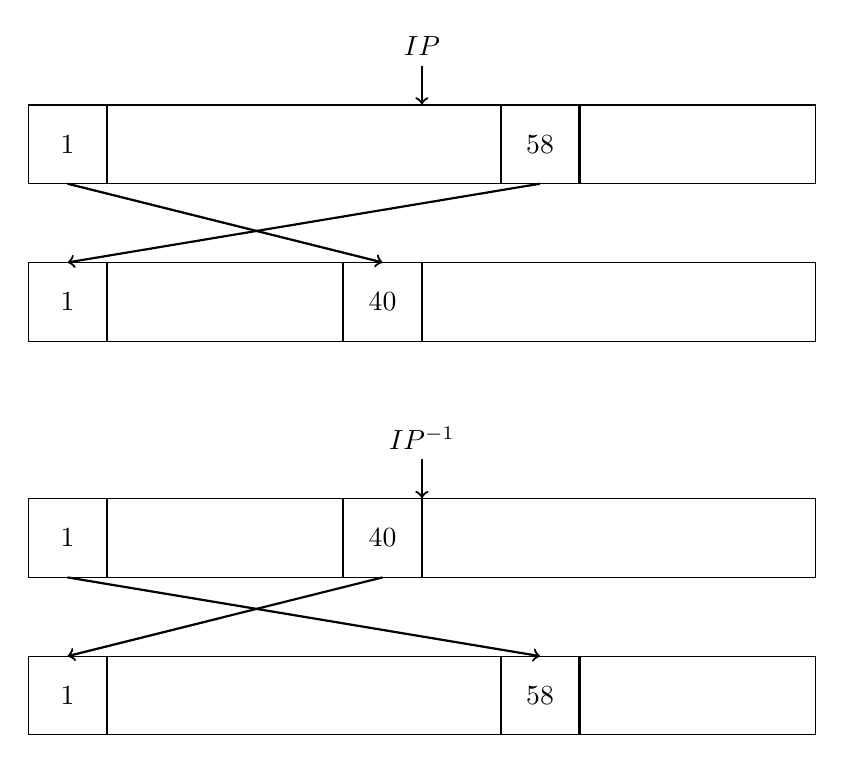
\begin{tikzpicture}
        % Boxes
        \node[anchor=south] at (5,-1) {$IP$};
        \node[draw, rectangle, minimum width=10cm, minimum height=1cm] (box1) at (5,-2) {};
        \node[draw, rectangle, minimum width=10cm, minimum height=1cm] (box2) at (5,-4) {};
        % lines and text in box1
        \node[anchor=center] at (0.5,-2) {1};
        \node[anchor=center] at (6.5,-2) {58};
        \draw[->, thick] (5,-1) -- (box1.north);
        \draw[-, thick] (1,-1.5) -- (1,-2.5);
        \draw[-, thick] (6,-1.5) -- (6,-2.5);
        \draw[-, thick] (7,-1.5) -- (7,-2.5);
        % lines bw the boxes
        \draw[->, thick] (0.5,-2.5) -- (4.5,-3.5);
        \draw[->, thick] (6.5,-2.5) -- (0.5,-3.5);
        % lines and text in box2
        \node[anchor=center] at (0.5,-4) {1};
        \node[anchor=center] at (4.5,-4) {40};
        \draw[-, thick] (1,-3.5) -- (1,-4.5);
        \draw[-, thick] (4,-3.5) -- (4,-4.5);
        \draw[-, thick] (5,-3.5) -- (5,-4.5);

        % Second set of boxes
        \node[anchor=south] at (5,-6) {$IP^{-1}$};
        \node[draw, rectangle, minimum width=10cm, minimum height=1cm] (box3) at (5,-7) {};
        \node[draw, rectangle, minimum width=10cm, minimum height=1cm] (box4) at (5,-9) {};
        % lines and text in box1
        \node[anchor=center] at (0.5,-7) {1};
        \node[anchor=center] at (4.5,-7) {40};
        \draw[->, thick] (5,-6) -- (box3.north);
        \draw[-, thick] (1,-6.5) -- (1,-7.5);
        \draw[-, thick] (4,-6.5) -- (4,-7.5);
        \draw[-, thick] (5,-6.5) -- (5,-7.5);
        % lines bw the boxes
        \draw[->, thick] (0.5,-7.5) -- (6.5,-8.5);
        \draw[->, thick] (4.5,-7.5) -- (0.5,-8.5);
        % lines and text in box2
        \node[anchor=center] at (0.5,-9) {1};
        \node[anchor=center] at (6.5,-9) {58};
        \draw[-, thick] (1,-8.5) -- (1,-9.5);
        \draw[-, thick] (6,-8.5) -- (6,-9.5);
        \draw[-, thick] (7,-8.5) -- (7,-9.5);

  \end{tikzpicture}
  \end{center}
  
    \centering   
  \end{figure}

\section*{Feistel Cipher}

% \begin{figure}[ht]
  \begin{figure}[ht]
  \begin{center}  
  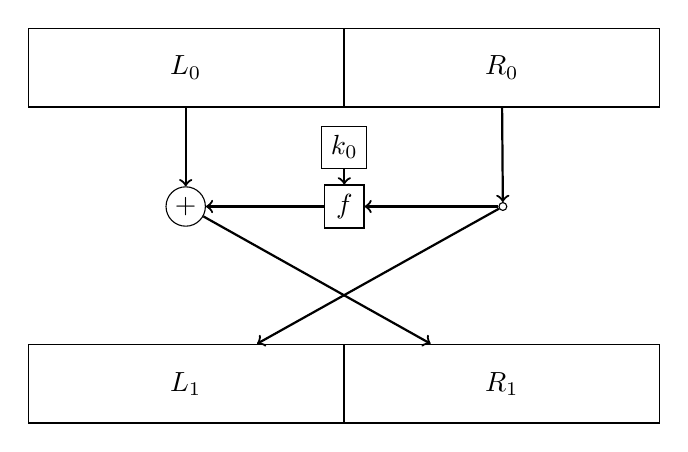
\begin{tikzpicture}[
    block1/.style={rectangle, draw, minimum width=4cm, minimum height=1cm, align=center},
    block2/.style={rectangle, draw, minimum width=0.5cm, minimum height=0.5cm, align=center},
    circlexor/.style={circle, draw, minimum size=0.5cm, inner sep=0pt},
    point/.style={circle, draw, minimum size=0.1cm, inner sep=0pt},
    arrow/.style={-Stealth, thick},
    node distance=2cm
  ]

    \node[block1] (L0) {$L_0$};
    \node[block1, right=0cm of L0] (R0) {$R_0$};
    \node[circlexor, below=1cm of L0] (xor) {+};
    \node[block1, below=3cm of L0] (L1) {$L_1$};
    \node[block1, right=0cm of L1] (R1) {$R_1$};
    \node[block2, right=1.5cm of xor] (f) {$f$};
    \node[block2, above=0.2cm of f] (k0) {$k_0$};
    \node[point, right=1.7cm of f] (point) {};

    \draw[->, thick] (L0) -- (xor);
    \draw[->, thick] (xor) -- (R1);
    \draw[->, thick] (R0) -- (point);
    \draw[->, thick] (point) -- (f);
    \draw[->, thick] (k0) -- (f);
    \draw[->, thick] (f) -- (xor);
    \draw[->, thick] (point) -- (L1);
  \end{tikzpicture}
  \end{center}
\end{figure}
% \end{figure}

% \begin{minipage}{0.45\textwidth}
  \begin{itemize}
    \item Left half(L0) is encrypted in one round and put on the right side(R1). 
    \item Right half(R0) is simply copied to the left side(L1). 
    \item The function f depends on the right half (here, R0) and the corresponding key of that round.
  \end{itemize}    
% \end{minipage}

\vspace*{100pt}
\subsection*{Function $f(K_{i+1},R_{i})$}

\begin{figure}[h!]
  \begin{center}
  \begin{tikzpicture}
        % Boxes
        \node[anchor=south] at (6,0) {$R_{i} (32 bit)$};
        \node[draw, rectangle, minimum width=2cm, minimum height=1cm] (box1) at (6,-1) {Expand};
        \draw[->, thick] (6,0) -- (box1.north);
        \node[draw, circle, minimum size=0.5cm] (xor1) at (6,-2.5) {$\oplus$};
        \node[anchor=west] at (7,-2.5) {$K_{i+1} (32 bit)$};\draw[->, thick] (7,-2.5) -- (xor1.east);
        \draw[->, thick] (box1.south) -- (xor1.north);\node[anchor=center] at (6.5,-3.5) {$48 bit$};
        % SUBSTITUTION PART
        \draw[-, thick] (xor1.south) -- (6,-4);
        \draw[-, thick] (0,-4) -- (12,-4);
        \draw[->, thick] (0,-4) -- (0,-5);\node[anchor=center] at (0.5,-4.5) {$6 bit$};
        \draw[->, thick] (1.5,-4) -- (1.5,-5);\node[anchor=center] at (2,-4.5) {$6 bit$};
        \draw[->, thick] (12,-4) -- (12,-5);\node[anchor=center] at (11.5,-4.5) {$6 bit$};
        %SUB BOXES
        \node[draw, rectangle, minimum width=1cm, minimum height=1cm] (s1) at (0,-6) {$S1$};
        \node[draw, rectangle, minimum width=1cm, minimum height=1cm] (s2) at (1.5,-6) {$S2$};
        \node[draw, rectangle, minimum width=1cm, minimum height=1cm] (s8) at (12,-6) {$S8$};
          %dots
          \fill[black] (3,-6) circle (1pt);
          \fill[black] (4.5,-6) circle (1pt);
          \fill[black] (6,-6) circle (1pt);
          \fill[black] (7.5,-6) circle (1pt);
          \fill[black] (9,-6) circle (1pt);
          \fill[black] (10.5,-6) circle (1pt);
        %lines again
        \node[draw, rectangle, minimum width=2cm, minimum height=1cm] (perm) at (6,-10) {$f(K_{i+1},R_{i})$};        
        \draw[->, thick] (6,-8) -- (perm.north);\node[anchor=center] at (6.5,-8.5) {$32 bit$};
        \draw[-, thick] (0,-8) -- (12,-8);
        \draw[-, thick] (0,-7) -- (0,-8);\node[anchor=center] at (0.5,-7.5) {$4 bit$};
        \draw[-, thick] (1.5,-7) -- (1.5,-8);\node[anchor=center] at (2,-7.5) {$4 bit$};
        \draw[-, thick] (12,-7) -- (12,-8);\node[anchor=center] at (11.5,-7.5) {$4 bit$};


  \end{tikzpicture}
  \end{center}
  
    \centering   
  \end{figure}

\subsection*{Expansion}
1 bit may expand to 1 or 2 bits.

\begin{figure}[ht]
  \begin{center}
  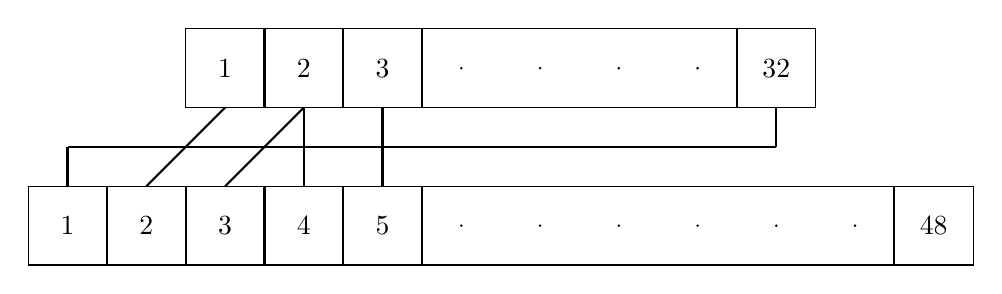
\begin{tikzpicture}
        % Boxes
        \node[draw, rectangle, minimum width=8cm, minimum height=1cm] (box1) at (6,0) {};
        \node[draw, rectangle, minimum width=12cm, minimum height=1cm] (box2) at (6,-2) {};
        % lines and text in box1
        \node[anchor=center] at (2.5,0) {1};
        \node[anchor=center] at (3.5,0) {2};
        \node[anchor=center] at (4.5,0) {3};
        \node[anchor=center] at (9.5,0) {32};
        \draw[-, thick] (3,0.5) -- (3,-0.5);
        \draw[-, thick] (4,0.5) -- (4,-0.5);
        \draw[-, thick] (5,0.5) -- (5,-0.5);
        \draw[-, thick] (9,0.5) -- (9,-0.5);
        % lines bw the boxes
        \draw[-, thick] (2.5,-0.5) -- (1.5,-1.5);
        \draw[-, thick] (3.5,-0.5) -- (2.5,-1.5);
        \draw[-, thick] (3.5,-0.5) -- (3.5,-1.5);
        \draw[-, thick] (4.5,-0.5) -- (4.5,-1.5);
        \draw[-, thick] (9.5,-0.5) -- (9.5,-1);
        \draw[-, thick] (0.5,-1) -- (9.5,-1);
        \draw[-, thick] (0.5,-1) -- (0.5,-1.5);

        % lines and text in box2
        \node[anchor=center] at (0.5,-2) {1};
        \node[anchor=center] at (1.5,-2) {2};
        \node[anchor=center] at (2.5,-2) {3};
        \node[anchor=center] at (3.5,-2) {4};
        \node[anchor=center] at (4.5,-2) {5};
        \node[anchor=center] at (11.5,-2) {48};
        \draw[-, thick] (1,-1.5) -- (1,-2.5);
        \draw[-, thick] (2,-1.5) -- (2,-2.5);
        \draw[-, thick] (3,-1.5) -- (3,-2.5);
        \draw[-, thick] (4,-1.5) -- (4,-2.5);
        \draw[-, thick] (5,-1.5) -- (5,-2.5);
        \draw[-, thick] (11,-1.5) -- (11,-2.5);
          %dots
          \fill[black] (5.5,0) circle (0.5pt);
          \fill[black] (6.5,0) circle (0.5pt);
          \fill[black] (7.5,0) circle (0.5pt);
          \fill[black] (8.5,0) circle (0.5pt);
          \fill[black] (6.5,-2) circle (0.5pt);
          \fill[black] (7.5,-2) circle (0.5pt);
          \fill[black] (8.5,-2) circle (0.5pt);
          \fill[black] (9.5,-2) circle (0.5pt);
          \fill[black] (10.5,-2) circle (0.5pt);
          \fill[black] (5.5,-2) circle (0.5pt);
        

  \end{tikzpicture}
  \end{center}
  
    \centering   
  \end{figure}

\subsection*{Substitution}
Substitution is done based on 8 tables(S1 to S8) of size 4$\times$16. The 6 bit input is used to navigate through the substitution table. The first and 
last bit indicates the row and the 4 bits in the middle indicate the column.

\clearpage
\noindent\tbox{
\begin{center}  
    \huge Lecture - 07 \\
    \Large Topic: Decryption of DES and Assymetric Cryptography
\end{center}
}

Last class we saw about encryption in DES. Now lets see how to decrypt it.
\section*{Decryption in DES}
For decryption we just follow the exact same enryption method in reverse order. You may think that we need to calculate $f^{-1}$ which had expansion and contraction using s-boxes.
But actually, we don't need its inverse and we can use the same $f$ function.\\
\begin{align*}
  R_{i+1} &= L_i \oplus f(k_i,R_i) \\
  L_i \oplus R_{i+1} &= L_i \oplus L_i \oplus f(k_i,R_i) \\
  L_i \oplus R_{i+1} &= f(k_i,R_i) \text{ [$R_i = L_{i+1}$]}\\
  L_i \oplus R_{i+1} &= f(k_i,L_{i+1}) \text{ [$R_i = L_{i+1}$]}\\
  L_i &= R_{i+1} \oplus f(k_i,L_{i+1}) \\
\end{align*}
Thus, we get $L_i$ from $R_{i+1}$ and $L_{i+1}$.

\begin{figure}[ht]
  \begin{center}  
  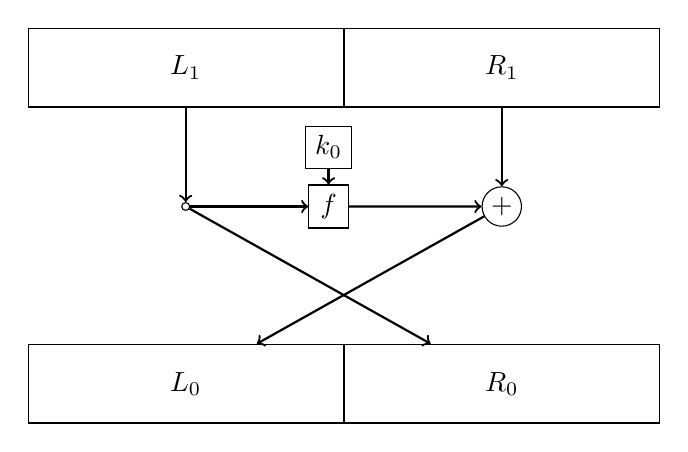
\begin{tikzpicture}[
    block1/.style={rectangle, draw, minimum width=4cm, minimum height=1cm, align=center},
    block2/.style={rectangle, draw, minimum width=0.5cm, minimum height=0.5cm, align=center},
    circlexor/.style={circle, draw, minimum size=0.5cm, inner sep=0pt},
    point/.style={circle, draw, minimum size=0.1cm, inner sep=0pt},
    arrow/.style={-Stealth, thick},
    node distance=2cm
  ]

    \node[block1] (L1) {$L_1$};
    \node[block1, right=0cm of L1] (R1) {$R_1$};
    \node[circlexor, below=1cm of R1] (xor) {+};
    \node[point, below=1.2cm of L1] (point) {};

    \node[block1, below=3cm of L1] (L0) {$L_0$};
    \node[block1, right=0cm of L0] (R0) {$R_0$};
    \node[block2, right=1.5cm of point] (f) {$f$};
    \node[block2, above=0.2cm of f] (k0) {$k_0$};

    \draw[->, thick] (R1) -- (xor);
    \draw[->, thick] (xor) -- (L0);
    \draw[->, thick] (L1) -- (point);
    \draw[->, thick] (point) -- (f);
    \draw[->, thick] (k0) -- (f);
    \draw[->, thick] (f) -- (xor);
    \draw[->, thick] (point) -- (R0);
  \end{tikzpicture}
  \end{center}
  \centering   
\end{figure}

As we have done the reverse, for 1 round, if we do it for 16 rounds, the final ouptut comes in $R_0$ and $L_0$ in reverse order and thus it should be reversed to get the original message.\\
Lets prove that its in reverse order. [d- denotes for bitstrings during decryption, and e- denotes encryption]
\begin{align*}
  L_0^d &= R_{16}^e \\
  R_0^d &= L_{16}^e = R_{15}^e \\
  L_1^d &= R_{0}^d = R_{15}^e \\
  R_1^d &= L_0^d \oplus f(R_0^d, k_1^d) \\
  &= L_0^d \oplus f(R_15^e, k_16^e) \\
  &= R_16^e \oplus f(R_15^e, k_16^e) \\
  &= L_15^e \oplus f(R_15^e, k_16^e) \oplus f(R_15^e, k_16^e) \\
  &= L_15^e \\
\end{align*}
thus, $R_1^d=L_15^e$ and similarly, $l_1^d=R_15^e$. so just the right and left are just reversed.

\section*{Probelem with DES, and subsequent methods}
Here, since the key length is just 64 bits, brute force method was very much possible, and so other methods such as AES, DES were introduced.\\
\subsection*{AES(Advanced Encryption Standard)}
AES is a block cipher which encrypts 128 bits at a time. Its key length are 128 bits, 192, or 256 in different different methods. Correspondigly, 10 rounds, 12, and 14 rounds of encryption happens respectively.\\
Unlike  DES, here every operation is byte(8 bits) wise and not bit wise.\\
In every round, the following happens:
\begin{itemize}
  \item byte Substitution(by passing thorough s-blocks and stuffs)
  \item Row shift (for diffusion)
  \item Mix column (for diffusion)
  \item Key addition(xor with key)
\end{itemize}
Since they are byte wise operation, (i.e, {0,1,2,..,255}) finite field algebra would be useful to understand AES.
Galois field theory (GF(256)) - prof suggested to read this on our own.

\subsection*{3DES or TDES(triple DES)}
It can be done is two ways as shown:

\begin{figure}[ht]
  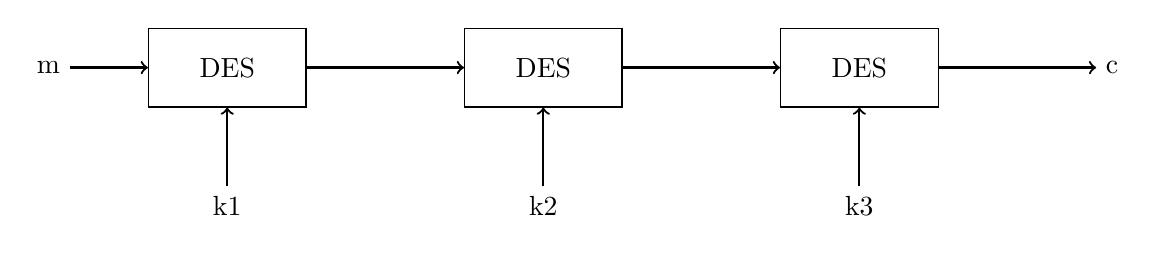
\begin{tikzpicture}
    % First set of text and boxes
    \node[anchor=east] (m) at (0,0) {m};
    \node[draw, rectangle, minimum width=2cm, minimum height=1cm] (des1) at (2,0) {DES};
    \node[draw, rectangle, minimum width=2cm, minimum height=1cm, right=2cm of des1] (des2) {DES};
    \node[draw, rectangle, minimum width=2cm, minimum height=1cm, right=2cm of des2] (des3) {DES};
    \node[right=2cm of des3] (c) {c};
    \node[below=1cm of des1] (k1) {k1};
    \node[below=1cm of des2] (k2) {k2};
    \node[below=1cm of des3] (k3) {k3};


    \draw[->, thick] (m) -- (des1.west);
    \draw[->, thick] (des1.east) -- (des2.west);
    \draw[->, thick] (des2.east) -- (des3.west);
    \draw[->, thick] (des3.east) -- (c);

    \draw[->, thick] (k1) -- (des1.south);
    \draw[->, thick] (k2) -- (des2.south);
    \draw[->, thick] (k3) -- (des3.south);

\end{tikzpicture}


  \centering   
\end{figure}

\begin{figure}[ht]
  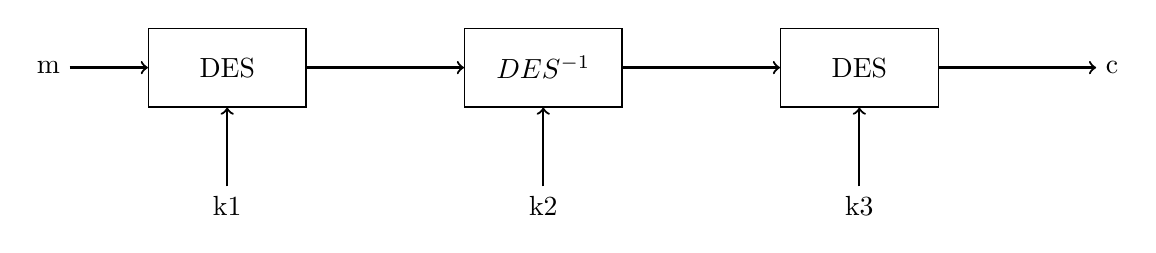
\begin{tikzpicture}
    % First set of text and boxes
    \node[anchor=east] (m) at (0,0) {m};
    \node[draw, rectangle, minimum width=2cm, minimum height=1cm] (des1) at (2,0) {DES};
    \node[draw, rectangle, minimum width=2cm, minimum height=1cm, right=2cm of des1] (des2) {$DES^{-1}$};
    \node[draw, rectangle, minimum width=2cm, minimum height=1cm, right=2cm of des2] (des3) {DES};
    \node[right=2cm of des3] (c) {c};
    \node[below=1cm of des1] (k1) {k1};
    \node[below=1cm of des2] (k2) {k2};
    \node[below=1cm of des3] (k3) {k3};


    \draw[->, thick] (m) -- (des1.west);
    \draw[->, thick] (des1.east) -- (des2.west);
    \draw[->, thick] (des2.east) -- (des3.west);
    \draw[->, thick] (des3.east) -- (c);

    \draw[->, thick] (k1) -- (des1.south);
    \draw[->, thick] (k2) -- (des2.south);
    \draw[->, thick] (k3) -- (des3.south);

\end{tikzpicture}


  \centering   
\end{figure}

\section*{Rivest–Shamir–Adleman (RSA) algorithm}
Its an Assymetric type encryption. The method is as follows.
\begin{itemize}
  \item get two large prime nos p and q (let $p,q > 2^1024$)
  \item find $n = pq$
  \item euler's function $\phi(n) = (p-1)(q-1)$
  \item select public key $e$ such that, $gcd(e,\phi(n) = 1)$
  \item obtain private key $d$ which is $= e^{-1} \pmod{\phi(n)} $. Here, inverse element exist because $gcd(e,\phi(n) = 1)$.
\end{itemize}
private info - d,p,q \\
public info - e,N
\begin{itemize}
  \item[encrypt:] $c = m^e \pmod{n}$
  \item[decrypt:] $c^d \pmod{n} = (m^e)^d \pmod{n} = m^{ed} \pmod{n} = m$ 
\end{itemize}
Generally, Assymetric key is computationally very expensive and thus very difficult to send the entire message through Assymetric method. Thus, keys of Symmetric key method are sent using Assymetric method and messages are sent with Symmetric key encryption henceforth.

\end{document}